\begin{titlepage}
  \newgeometry{top=3cm, bottom=3cm, left=2.25 cm, right=2.25cm}	% Temporarily change margins		

  % TODO: Change figure.
  % Cover picture (replace with your own or delete)		
  \begin{figure}[H]
    \centering
    \vspace{2cm}	% Adjust vertical spacing here
    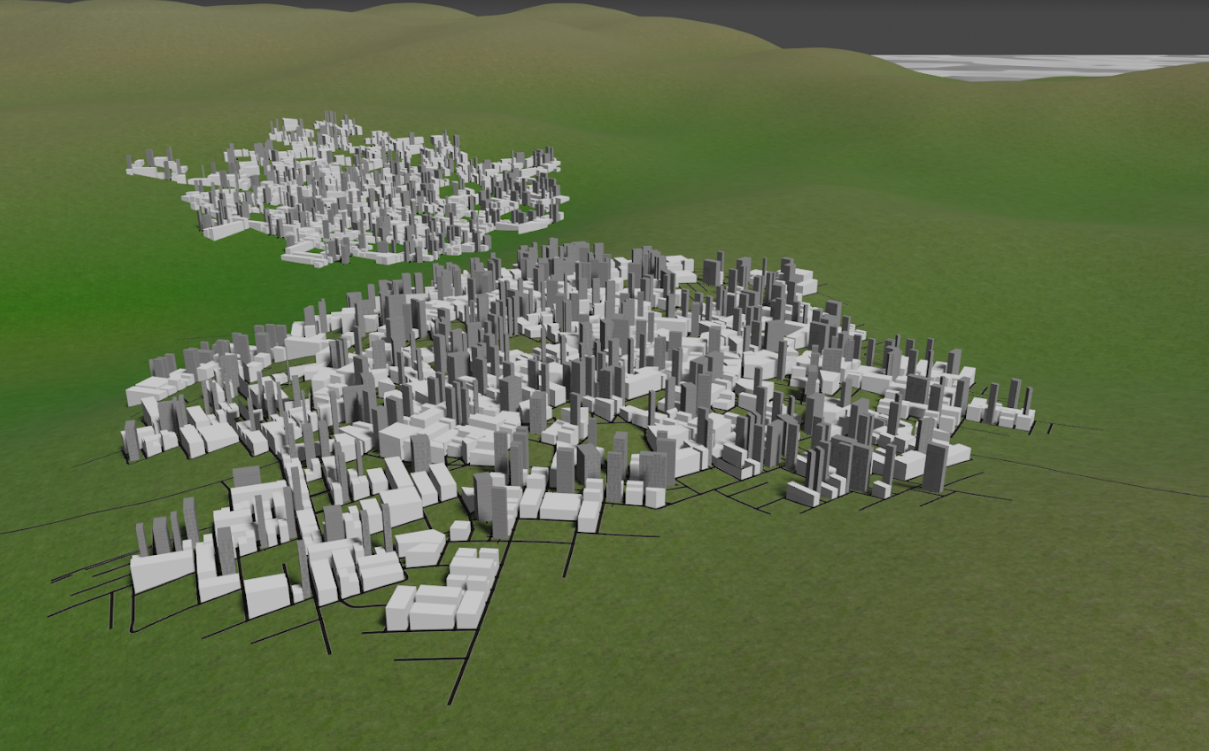
\includegraphics[width=1\linewidth]{figure/cover.png}
  \end{figure}

  % Cover text
  \renewcommand{\familydefault}{\sfdefault} \normalfont % Set cover page font
  \textbf{{\Huge Procedural Generation of Modern 3D Cities}} 	\\[0.5cm]
  Bachelor's thesis in Computer Science and Engineering \setlength{\parskip}{1cm}

  {\Large
    Theodor Angergård \\[0.1cm]
    Marcus Ansamaa \\[0.1cm]
    Alexander Arvidsson \\[0.1cm]
    Jacob Eriksson \\[0.1cm]
    Anton Håkansson \\[0.1cm]
    Viktor Truvé \\[0.1cm]
  }

  Department of Computer Science and Engineering \\
  \textsc{Chalmers University of Technology} \\
  Gothenburg, Sweden \the\year

  \renewcommand{\familydefault}{\rmdefault} \normalfont % Reset standard font
  \vfill	
\end{titlepage}

% BACK OF COVER PAGE (BLANK PAGE)
\newpage
\restoregeometry
\thispagestyle{empty}
\mbox{}


% TITLE PAGE
\newpage
\thispagestyle{empty}
\begin{center}
  \textsc{\large Bachelor of Science Thesis \the\year}\\[4cm]		% Report number given by department 
  \textbf{\Large Procedural Generation of Modern 3D Cities} \\[1cm]
  {\Large
    Theodor Angergård \\[0.1cm]
    Marcus Ansamaa \\[0.1cm]
    Alexander Arvidsson \\[0.1cm]
    Jacob Eriksson \\[0.1cm]
    Anton Håkansson \\[0.1cm]
    Viktor Truvé \\[0.1cm]
  }    
  \vfill	

  % Logotype on titlepage	
  \begin{figure}[H]
    \centering
    % Remove the following line to remove the titlepage logotype
    
\includegraphics[width=0.2\pdfpagewidth]{figure/chalmers.png} \\	
  \end{figure}	\vspace{5mm}	
  
  Department of Computer Science and Engineering \\
  \textsc{Chalmers University of Technology} \\
  Gothenburg, Sweden \the\year \\
\end{center}


% IMPRINT PAGE (BACK OF TITLE PAGE)
\newpage
\thispagestyle{empty}
\vspace*{4.5cm}
\textbf{Procedural Generation of Modern 3D Cities} \\
Theodor Angergård \\
Marcus Ansamaa \\
Alexander Arvidsson \\
Jacob Eriksson \\
Anton Håkansson \\
Viktor Truvé \\
\setlength{\parskip}{1cm}

\copyright ~ Theodor Angergård, 2020 \\
\copyright ~ Marcus Ansamaa, 2020 \\
\copyright ~ Alexander Arvidsson, 2020 \\
\copyright ~ Jacob Eriksson, 2020 \\
\copyright ~ Anton Håkansson, 2020 \\
\copyright ~ Viktor Truvé, 2020 \\

Supervisor: Staffan Björk, Department of Interaction Design and Technologies \\
Examiner: Michael Heron, Department of Computer Science and Engineering \setlength{\parskip}{1cm}

Bachelor's Thesis \the\year\\	% Report number given by department 
Department of Computer Science and Engineering\\
Chalmers University of Technology\\
SE-412 96 Gothenburg\\
Telephone +46 31 772 1000 \setlength{\parskip}{0.5cm}

\vfill
% Caption for cover page figure if used, possibly with reference to further information in the report
Cover: A 3D city model that was generated and exported with CityCraft. The rendering of the model was done in Blender. \setlength{\parskip}{0.5cm} \\
Typeset in \LaTeX \\
Gothenburg, Sweden \the\year